\subsubsection{Korekcja (patching) łańcuchów znaków (Win32)}

Możemy w łatwy sposób znaleźć łańcuch znaków  \q{hello, world} w pliku wykonywalnym za pomocą Hiew:

\begin{figure}[H]
\centering
\myincludegraphics{patterns/01_helloworld/hola_edit1.png}
\caption{Hiew}
\label{}
\end{figure}

Możemy przetłumaczyć naszą wiadomość na język hiszpański:

\begin{figure}[H]
\centering
\myincludegraphics{patterns/01_helloworld/hola_edit2.png}
\caption{Hiew}
\label{}
\end{figure}

Tekst w języku hiszpańskim jest o 1 bajt krótszy od tekstu w języku angielskim, dlatego dodajemy na koniec bajt 0x0A (\TT{\textbackslash{}n}) i bajt zerowy.

Działa.

A co jeśli chcielibyśmy wstawić dłuższy tekst?
Po oryginalnym tekście w języku angielskim widzimy kilka bajtów zerowych.
Trudno powiedzieć czy można je nadpisać: mogą (ale nie muszą!) one być wykorzystywane gdzieś w kodzie \ac{CRT}.
Tak czy inaczej, możemy je nadpisywać tylko jeśli naprawdę wiemy co robimy.

\subsubsection{Korekcja łańcuchów znaków (Linux x64)}

\myindex{\radare}
Spróbujmy edytować plik wykonywalny systemu Linux x64, korzystając z \radare{}:

\lstinputlisting[caption=Sesja w \radare{}]{patterns/01_helloworld/radare.lst}

Co tu  się dzieje: szukam łańcucha znaków \q{hello}, korzystając z komendy \TT{/},
następnie ustawiam \emph{kursor} (\emph{seek} w terminologii \radare{}) pod ten adres.
Następnie chcę się upewnić, że jest to rzeczywiście poszukiwane miejsce: \TT{px} wyświetla bajty pod tym adresem.
\TT{oo+} przełącza \radare{} w tryb \emph{odczytu/zapis}.
\TT{w} zapisuje łańuch znaków ASCII w miejscu kursora (\emph{seek}).
Warto zauważyć \TT{\textbackslash{}00} na końcu, jest to bajt zerowy.
\TT{q} wyłącza \radare.


\subsubsection{Prawdziwa historia crackowania oprogramowania}
\myindex{\SoftwareCracking}

Program do przetwarzania obrazów, niezarejestrowany, dodawał do pliku znak wodny,
na przykład napis \q{This image was processed by evaluation version of [nazwa oprogramowania]}
Spróbowaliśmy najprostszego rozwiązania: znaleźliśmy ten tekst w pliku wykonywalnym i zastąpiliśmy go spacjami.
Znak wodny zniknął.
Ogólnie rzecz biorąc, wciąż był nakładany przez program.
\myindex{Qt}
Za pomocą funkcji Qt, znak wodny wciąż był dodawany do obrazu.
Ale dodawanie spacji nie zmieniało go w żaden sposób...

\subsubsection{Tłumaczenie oprogramowania za czasów MS-DOS}
\myindex{MS-DOS}

Sposób przedstawiony wyżej był powszechnie wykorzystywany w latach 80. i 90. przy tłumaczeniu oprogramowania pod MS-DOS na język rosyjski.
Ta technika może być wykorzystywana przy braku wiedzy na temat kodu maszynowego i formatów plików wykonywalnych.
Nowy łańcuch znaków nie powinien być dłuższy niż stary, ponieważ istnieje ryzyko nadpisania innej wartości albo fragmentu kodu wykonywalnego

Rosyjskie słowa i zdania zwykle są trochę dłuższe od angielskich odpowiedników, dlatego \emph{przetłumaczone} oprogramowanie zawierało
sporo dziwnych akronimów (skrótowców) i trudnych do zrozumienia skrótów.

\begin{figure}[H]
\centering
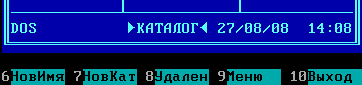
\includegraphics[width=0.5\textwidth]{patterns/01_helloworld/Norton_Commander_v5_51.png}
\caption{Norton Commander 5.51 przetłumaczony na język rosyjski}
\end{figure}
% note to translators: if you know such examples of MS-DOS programs 'localized' to your native language,
% please tell me, maybe I will add more screenshots.

Prawdopodobnie sytuacja wyglądała podobnie z tłumaczeniem na inne języki.

\myindex{Borland Delphi}
W przypadku łańcuch znaków w Delphi, rozmiar również musi być poprawiony, jeśli zachodzi taka potrzeba.



